\section{Theorie}
\label{sec:Theorie}
In einer evakuierten Röhre werden aus einer Glühkatode emittierte Elektronen auf eine Anode hin beschleunigt.
Beim Auftreffen auf die Anode entsteht Röntgenstrahlung , die sich aus dem kontinuierlichen Bremsspektrum
und der charakteristischen Röntgenstrahlung des Anodenmaterials zusammensetzt.
Durch die Abbremsung eines Elektrons im Coulombfeld des Atomkerns wird ein Photon,
dessen Energie dem Energieverlust des abgebremsten Elektrons entspricht,
ausgesendet.
Das Bremsspektrum ist kontinuierlich, weil das Elektron sowohl einen Teil, als auch seine gesamte kinetische Energie abgeben kann.
Die maximale Energie bzw. minimale Wellenlänge
\begin{equation}
    \lambda = \frac{h \cdot c}{e_0 U}
    \label{eqn:gl1}
\end{equation}
ergibt sich bei der vollständigen Abbremsung des Elektrons.
\begin{figure}
    \centering
    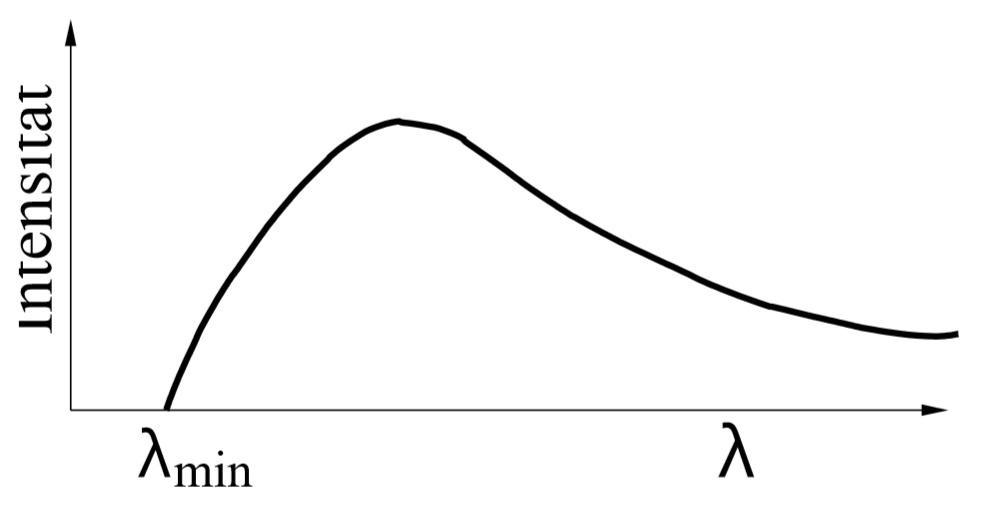
\includegraphics[height=4.0cm]{data/abb1.jpg}
    \caption{Bremsspektrum \cite{V602}}
    \label{fig:abb1}
\end{figure} \\
\noindent
Hierbei wird die gesamte kinetische Energie $E_{\text{kin}} = e_0 U$ in Strahlungsenergie $E = h \cdot \nu$ umgewandelt.\\
\noindent
Durch das Ioniesieren des Anodenmaterials, so dass eine Leerstelle in einer inneren Schale entsteht, kann ein Elektron einer äußeren Schale unter Aussendung eines Röntgenquants in die innere Schale zurückfallen.
Das charakteristische Spektrum besteht aus scharfen Linien, weil beim Zurückfallen genau die Energiedifferenz zwischen den beiden Energieniveaus der beiden Schalen $h \nu = E_{\text{m}} - E_{\text{n}}$ freigesetzt wird.
Diese Diferenz ist charakteristisch für verschiedene Anodenmaterialien.
Die einzelnen Linien werden mit $\text{K}_{\alpha}, \text{K}_{\beta}, \text{L}_{\alpha},...$ bezeichnet, wobei die Buchstaben K,L,M,... die Schale bezeichnen, auf der die Übergänge enden.
Dem griechischem Buchstaben kann man entnehmen, woher das beteiligte äußere Elektron stammt.
In einem Mehrelektronenatom schirmen die Hüllenelektronen und die Wechselwirkung der Elektronen untereinander die Kernladung ab.
Dies führt zu einer Verringerung der Coulomb Anziehung auf das äußere Elektron, sodass für die Bindungsenergie $E_\text{n}$ eines Elektrons auf der n-ten Schale gilt:
\begin{equation}
    E_\text{n} = -R_{\infty}z_{\text{eff}}^2 \cdot \frac{1}{n^2}
    \label{eqn:gl2}
\end{equation}
Der Abschirmeffekt wird durch die effektive Kernladung $z_{\text{eff}} = z - \sigma$ berücksichtigt.
\sigma ist die Abschirmkonstante und $R_{\infty} = 13,6 \text{eV}$ ist die Rydbergenergie.
Da die äußeren Elektronen aufgrund des Bahndrehimpulses und des Elektronenspins nicht alle dieselbe Bindungsenergie besitzen, ist in der Regel jede charakteristische Linie in eine Reihe von eng beieinander liegenden Linien aufgelöst (Feinstruktur).
Diese können in dem vorliegenden Versuchsaufbau nicht aufgespalten werden.
Bei der im Versuch verwendeten Kupferanode können die $\text{Cu-K}_{\alpha}\text{- und die Cu-K}_{\beta}\text{-Linien}$ beobachtet werden, die der Bremsstrahlung überlagert sind.\\
\noindent
Bei der Absorption von Röntgenstrahlung unter 1 MeV sind der Photoeffekt und der Comptoneffekt die dominanten Prozesse.
Mit zunehmender Energie nimmt der Absorptionskoeffizient ab und steigt sprunghaft an, wenn die Photoenergie gerade größer ist als die Bindungsenergie eines Elektrons aus der nächst inneren Schale.
Die Lage der Absorptionskanten $h \nu_{\text{abs}} = E_{\text{n}} - E_{\infty}$ ist nahezu identisch mit der Bindungsenergie.
Je nachdem aus welcher Schale das Elektron stammt, wird die zugehörige Absorptionskante K-, L-, M-,... als Absorptionskante bezeichnet.
Aufgrund der Feinstrukturen werden drei L-Kanten beobachtet, aber nur eine K-Kante.
\begin{figure}
    \centering
    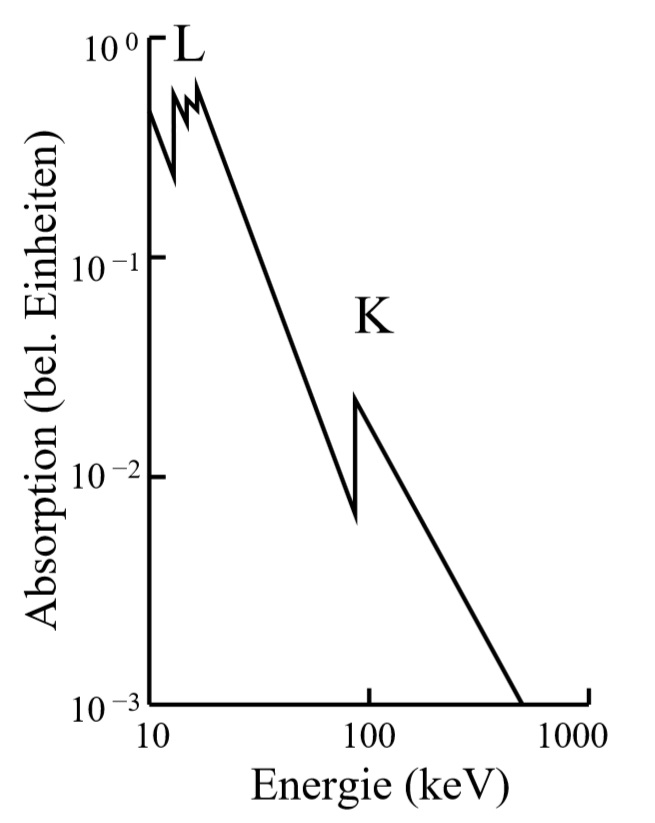
\includegraphics[height=4.0cm]{data/abb2.jpg}
    \caption{Absorptionsspektrum \cite{V602}}
    \label{fig:abb2}
\end{figure} \\
\noindent
Die Bindungsenergie $E_{n,j}$ eines Elektrons muss aufgrund der Feinstrukturen mit der Sommerfeldschen Feinstrukturformel berechnet werden.
\begin{equation}
    E_{n,j} = -R_{\infty}\left(z_{\text{eff}}^2 \cdot \frac{1}{n^2} + \alpha^2 z_{\text{eff,2}}^4 \cdot \frac{1}{n^3} \left( \frac{1}{j + \frac{1}{2}} - \frac{3}{4n}\right)\right)
    \label{eqn:gl3}
\end{equation}
n ist die Hauptquantenzahl, \alpha die Sommerfeldsche Feinstrukturkonstante und j der Gesamtdrehimpuls.
Bei der Bestimmung der Abschirmkonstante ${\sigma}_L$ aus der L-Kante müssen die Abschirmzahlen jedes beteiligten Elektrons berücksichtigt werden.
Die Rechnung wird vereinfacht durch bestimmung der Energiedifferenz $\Delta E_{\text{L}}$ zweier L-Kanten.
Im Vorliegenden Versuch können die $\text{L}_1- \text{und L}_2-$Kante nicht aufgelöst werden, so dass sich ${\sigma}_L$
\begin{equation}
    {\sigma}_L = Z - \left(\frac{4}{\alpha}\sqrt{\frac{\Delta E_{\text{L}}}{R_{\infty}}} - \frac{5 \Delta E_{\text{L}}}{R_{\infty}}\right)^{1/2}\left(1 + \frac{19}{32}\alpha^2\frac{\Delta E_{\text{L}}}{R_{\infty}}\right)^{1/2}
    \label{eqn:gl4}
\end{equation}
aus der Energiedifferenz $\Delta E_{\text{L}} = E_{\text{$\text{L}_2$}} - E_{\text{$\text{L}_3$}}$ und der Ordnungszahl $Z$ bestimmen lässt.
Durch die Braggsche Reflexion kann die Energie E bzw. Wellenlänge \lambda experimentell analysiert werden.
\begin{figure}
    \centering
    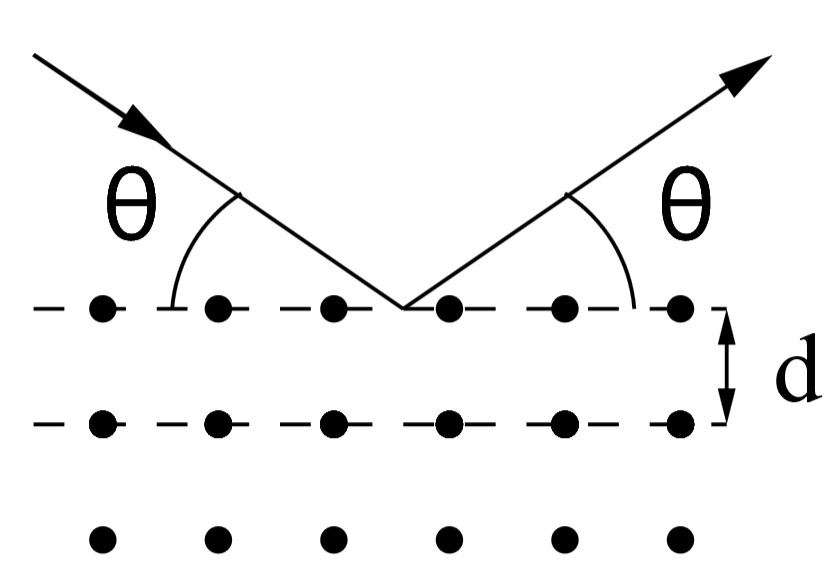
\includegraphics[height=4.0cm]{data/abb3.jpg}
    \caption{Braggsche Reflexion am Gitter \cite{V602}}
    \label{fig:abb3}
\end{figure} \\
\noindent
Die Photonen werden an jedem Atom des Gitters (z.B. ein LiF-Kristall) gebeugt.
Die Röntgenstrahlen interferieren miteinander und beim Glanzwinkel \Theta erhält man konstruktive Interferenz.
Bei bekannter Gitterkonstante d kann mit Hilfe der Braggschen Bedingung
\begin{equation}
    2 d \sin{\Theta} = n \lambda
\end{equation}
aus dem Winkel \Theta die gebeugt Wellenlänge \lambda bestimmt werden, wobei n die Beugungsordnung ist.

\section{Aufbau}
\label{sec:aufbau}
\begin{figure}
    \centering
    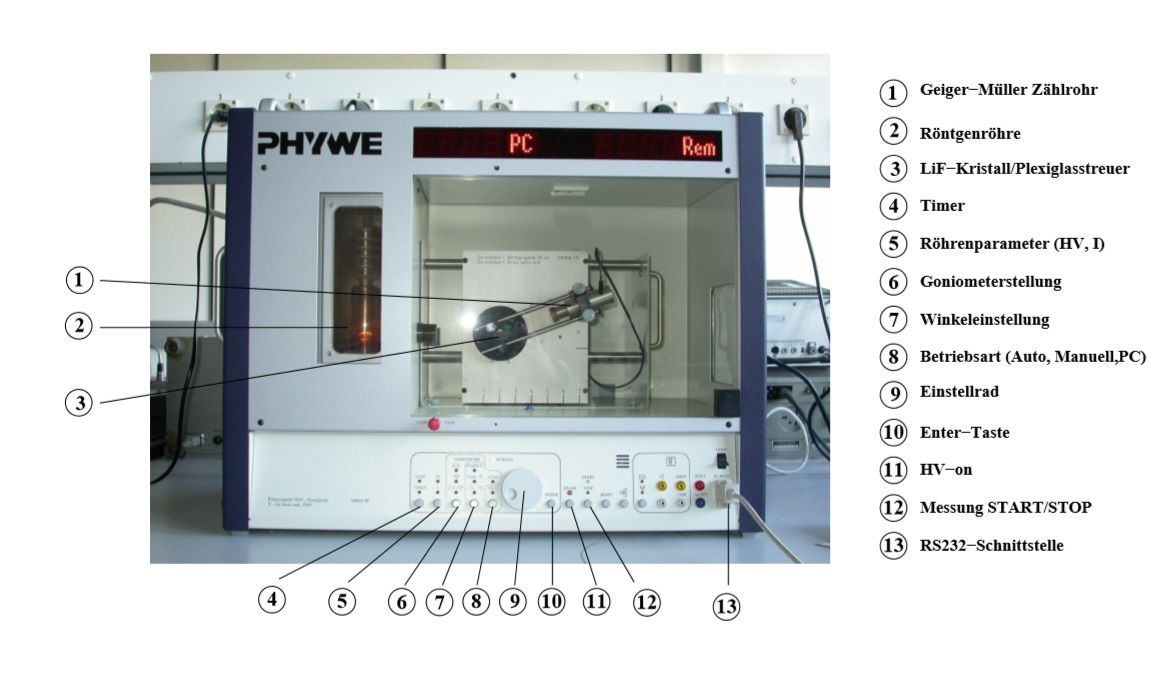
\includegraphics[height=6.0cm]{data/abb4.jpg}
    \caption{Versuchsaufbau \cite{V602}}
    \label{fig:abb4}
\end{figure}
\noindent
Es wird eine Kupfer-Röntgenröhre, ein LiF-Kristall und ein Geiger-Müller-Zählrohr benötigt.
Die Elektronik ist im Röntgengerät (Abb. \ref{fig:abb4}) integriert.
Über die Menüpunkte kann die Messart, der Drehmodus, der Kristallwinkel, sowie die Integrationszeit gewählt und die Messung gestartet werden.
Die Beschleunigungsspannung wird auf $U_\text{B} = 35 \text{kV}$ und der Emissionsstrom auf $I = 1 \text{mA}$.
Die 1 mm Blende und der LiF-Kristall werden in die Halterungen gesteckt und die Schlitzblende muss waagerecht auf dem Geiger-Müller Zählrohr sitzen.
Für die Absorptionsmessungen können Blenden mit verschiedenen Absorbern vor das Geiger-Müller Zählrohr geschraubt werden.
